\documentclass[10pt,twocolumn,letterpaper]{article}

\usepackage{cvpr}
\usepackage{times}
\usepackage{epsfig}
\usepackage{graphicx}
\usepackage{amsmath}
\usepackage{amssymb}

\usepackage{url}

% Include other packages here, before hyperref.
\usepackage{algorithm}
\usepackage{algpseudocode}
\usepackage{xcolor}

% If you comment hyperref and then uncomment it, you should delete
% egpaper.aux before re-running latex.  (Or just hit 'q' on the first latex
% run, let it finish, and you should be clear).
%\usepackage[pagebackref=true,breaklinks=true,letterpaper=true,colorlinks,bookmarks=false]{hyperref}

\cvprfinalcopy % *** Uncomment this line for the final submission

\def\cvprPaperID{****} % *** Enter the CVPR Paper ID here
\def\httilde{\mbox{\tt\raisebox{-.5ex}{\symbol{126}}}}

% Pages are numbered in submission mode, and unnumbered in camera-ready
\ifcvprfinal\pagestyle{empty}\fi
\begin{document}

%%%%%%%%% TITLE
\title{Local Binary Pattern: comparison between a sequential and parallel implementation}

\author{Beatrice Paoli\\
{\tt\small beatrice.paoli@stud.unifi.it}
}

\maketitle
\thispagestyle{empty}

%%%%%%%%% ABSTRACT
\begin{abstract}
%The purpose of this paper is to implement the algorithm to compute the Local Binary Pattern for an image. There are many variations of this algorithm: the chosen implementation allows to choose any radius and number of pixels in the neighborhood but does not consider "uniform patterns". Both a sequential and a parallel implementation are presented and the two versions are compared in terms of execution times and speedup. The implementations are done in Python and the parallel version uses the Joblib package.
The purpose of this paper is to implement the algorithm to compute the Local Binary Pattern for an image. There are many variations of this algorithm: the chosen implementation allows to choose any radius and number of pixels in the neighborhood and considers "uniform patterns" for labelling each pixel of the image. Both a sequential and a parallel implementation are presented and the two versions are compared in terms of execution times and speedup. The implementations are done in Python and the parallel version uses the Joblib package.
\end{abstract}

%-------------------------------------------------------------------------

\section{Introduction}
Local Binary Pattern (LBP) is a simple and efficient texture descriptor that labels each pixel of an image with a binary number based on the neighboring pixels in order to create a local representation of the texture.

Used for texture analysis and classification, thanks to its computational simplicity it is widely used for many applications such as face analysis and motion analysis.

Many variants have been developed over time, but the basic idea of the LBP operator is to assign to each pixel of the greyscaled image a value by 
considering the difference of each of the 3x3 neighboring pixels with the center as binary values and then combine them in a clockwise or counter-clockwise to get the decimal label to assign to the pixel.

The histogram obtained from the occurrencies of these $2^8$ labels can be used as a texture descriptor.

An extension of this basic concept allows to use circular neighborhoods of different sizes and different distances from the center. The operator is denoted as $LBP_{P, R}$ where $P$ is the number of sampled neighbors and $R$ is the radius of the circle where the sampled pixels stand.

If $c_x$ and $c_y$ are the coordinates of the center pixel, the coordinates of each neighbour pixel $p$ can be computed as:

\begin{gather*}
	p_x = c_x - R\sin(2\pi p/P) \\ 
	p_y = c_y + R\cos(2\pi p/P)
\end{gather*}

If these coordinates don't end into the center of a pixel, the grayscale value is bilinearly interpolated.

At this point, the LBP operator is computed as:

\[LBP_{P, R} = \sum_{p = 0}^{P - 1}s(g_p - g_c)2^p\]

where $g_c$ and $g_p$ are respectively the grayscale values of the center pixel and neighbouring pixel and:

\[s(x) = \begin{cases} 1, & \mbox{if } x \ge 0 \\ 0, & \mbox{otherwhise} \end{cases}\]

This version of the LBP operator is not rotation-invariant as it depends on the order of consideration of the $0...P-1$ neighbours. So rotating the image will lead to different results.

%To solve this problem, another variant of the LBP operator considers \textit{uniform patterns} to achieve rotation-invariance, but for the implementation presented in this paper it wasn't used.

To solve this problem, another variant of the LBP operator considers \textit{uniform patterns} to achieve rotation-invariance. A circular neighbourhood of pixels is said to have a uniform pattern if there are few spatial transitions.

More formally, we define the function $U$ that calculates the number of spatial transitions (bitwise 0/1 changes) in the neighbourhood pattern.

Only patterns with a value of $U$ of at most 2 are considered uniform. With this, a new definition of the LBP operator is given.

\[LBP_{P, R}^{riu2} = \begin{cases} \sum_{p = 0}^{P - 1}s(g_p - g_c), & \mbox{if } U(LBP_{P, R}) \le 2 \\ P + 1, & \mbox{otherwhise} \end{cases}\]

where

\begin{equation*}
	\begin{split} 
		U(LBP_{P, R}) & = |s(g_{p - 1} - g_c) - s(g_0 - g_c)| \\ & + \sum_{p = 1}^{P - 1}|s(g_p - g_c) - s(g_{p -1} - g_c)|
	\end{split}
\end{equation*}

This reduces the number of possible labels to $P + 2$ values.

After obtaining the labeled image $f_l(x, y)$ the LBP histogram can be defined as:

\[H_i = \sum_{x, y}I\{f_l(x, y) = i\}, i = 0...n -1\]

where n is the number of different labels assigned and:

\[I(A) = \begin{cases} 1, & \mbox{if } A \mbox{ is true} \\ 0, & \mbox{otherwhise} \end{cases}\]

If we need to compare histograms of images of different sizes, they must be normalized first:

\[N_i = \frac{H_i}{\sum_{j = 0}^{n - 1}H_j}\]

\section{Implementation}

The implementation is done in Python and uses the \textit{Pillow} package to load and save images in RGB format, and the \textit{numpy} package for handling arrays. 

The application first loads the image in grayscale and converts it into a numpy array.

In the LBP function, the image is padded by adding a frame of pixels with the constant value of 0 and is done by using the numpy function \verb"pad". This is necessary for the computation of the LBP labels of the edges and to allow any radius to be used as a parameter. The size of the padding on each side is $R$ rounded up to the nearest integer.

The LBP labels are then computed with the use of uniform patterns.
To bilinearly interpolate the grayscale value $g_p$ at $(p_x, p_y)$, the following formula is used:

\begin{equation*}
	\begin{split} 
		g_p & = \frac{1}{(x_2 - x_1)(y_2 - y_1)} \cdot \\ &
		\begin{bmatrix}
			x_2 - p_x & p_x - x_1
		\end{bmatrix}
		\begin{bmatrix}
			Q_{11} & Q_{12} \\
			Q_{21} & Q_{22}
		\end{bmatrix}
		\begin{bmatrix}
			y_2 - p_y \\ 
			p_y - y_1
		\end{bmatrix}
	\end{split}
\end{equation*}


where $Q_{11} = (x_1, y_1), \quad Q_{12} = (x_1, y_2), \quad Q_{21} = (x_2, y_1), \quad Q_{22} = (x_2, y_2)$ are respectively the bottom-left, top-left, bottom-right and top-right closest valid pixel values to $(p_x, p_y)$.

The pseudo-code of the LBP function is the following:

\begin{algorithm}[H]
	\caption{Local Binary Pattern}
	\label{alg:lbp}
	\begin{algorithmic}
		\Require input image, P, R
		\vspace{0.5cm}
		
		\State Pad input image
		\For{$cy \in [0...height)$}
		\For{$cx \in [0...width$)}
		\State $lbp\_val \leftarrow 0$
		\For{$p \in [0...P)$}
		\State $p_x \leftarrow c_x - R\sin(2\pi p/P)$
		\State $p_y \leftarrow c_y + R\cos(2\pi p/P)$
		\If{$p_x, p_y$ are integers}
		\State $g_p \leftarrow input(p_x, p_y)$
		\Else
		\State $g_p \leftarrow bilinear\_interpolation(p_x, p_y)$
		\EndIf
		\If{$g_p \ge g_c$}
		\State $lbp\_val \leftarrow lbp\_val + 1$
		\EndIf
		\EndFor
		\State $u \leftarrow U(LBP_{P, R})$
		\If{$u > 2$}
		\State $lbp\_val \leftarrow P + 1$
		\EndIf
		\State $output(c_x, c_y) \leftarrow lbp\_val$
		\EndFor
		\EndFor
		\State \Return output image
		
	\end{algorithmic}
\end{algorithm}

Finally, the output array is used to compute the histogram and then both histogram and image are saved on a file. 

\section{Parallelization}

The computation of the output label for each pixel only requires to read some pixels from the input image. The only write operation necessary is the assignment of the label to the output pixel and they are all independent from each other. 

Therefore, this is an embarassingly parallel problem: each output pixel can be computed by a thread without the need of any synchronization.

The Python interpreter is based on the \textit{Global Interpreter Lock} (GIL), which prevents the execution of multiple threads. To bypass this problem and achieve parallelization, we need to use processes instead of threads.
Each process will have its own interpreter (including its own GIL) and  memory, so their instantiation has a greater overhead compared to threads.

For this implementation, the \textit{Joblib} library was used. It is a high level library that allows to parallelize computation through the use of a backend library (\textit{multiprocessing} or \textit{loki}) in a transparent way.

While tecnically each output pixel could be computed independently, it isn't convenient to spawn too many processess, nor to fraction a process job in too many parts. 

Therefore the image is split in a number of sub-images equal to the number of processes to use. So each process computes only an output slice of the total output. The split and join is performed by the main process.

Each processes needs in input the image, the parameters $P$ and $R$ and the indices of the output sub-image. Each subprocess first performes some checks to avoid going out of bound and then computes the padded array (numpy's \verb"pad" is extremely fast, no slowdown is caused by having this computation repeated for each process).

However, the only problem is represented by the input array which can be very big and can result to a very slow instantiation of the processess due to the array copy. This problem can be solved by using the \verb"joblib.dump()" and \verb"joblib.load()" functions to save and reload the numpy array efficiently. 

The main process saves the array on disk and deletes it at the end of the function, while each process loads the file to perform the lbp operator on its slice of the image. 

To recap, the main process:

\begin{enumerate}
	\item Saves the input array on disk in a compressed format.
	\item Splits the original image in sub-images.
	\item Instantiates the sub-processes with the \verb"Parallel" class, each with their own parameters.
	\item After all sub-processess terminate, the output image is built from the returned slices.
\end{enumerate}

The work of each subprocess is similar to the one described in Algorithm \ref{alg:lbp}, the only things that changes are the for loops that only iterate on the assigned slice and the necessary shifting of some pixel coordinates. 

\section{Performance Analysis}
In order to compare the performance of a sequential algorithm with its parallel version we can use the concept of \textit{speedup}.

Speedup is measured as the ratio between the execution time of the sequential algorithm and the parallel one.

\[S = \frac{t_s}{t_p}\]

Ideally, we should look for \textit{perfect speedup} or even \textit{linear speedup}, meaning $S$ should be equal or similar to the number of processors used to perform the parallel algorithm.

The tests were performed on a Intel Core i7-1165G7 with 4 physical cores and 8 logical cores. To evaluate the application performance, images of different sizes and different values for the parameter $P$ were used.

The parameter $R$ is not considered since its variation doesn't cause any change in execution times and speedup.

\begin{figure}[H]
	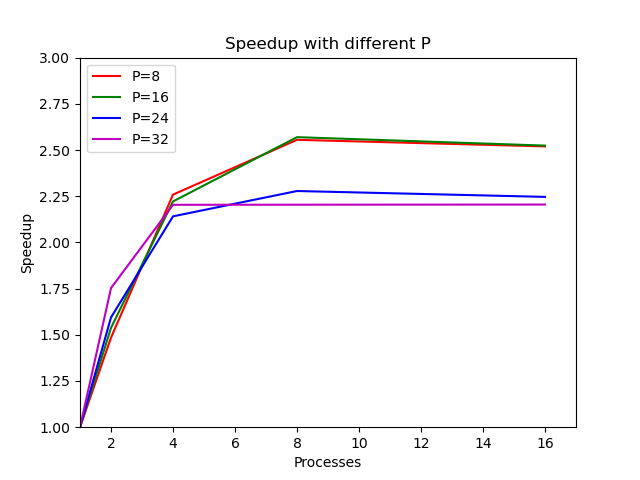
\includegraphics[width=\linewidth]{images/speedup_by_p.png}
	\caption{Speedup of the LBP operator on a 734x694 image and $R = 1$ with different values for P.}
	\label{fig:speedup_kernel}
\end{figure}

\begin{table}[H]
	\begin{center}
		\begin{tabular}{|c|c|c|}
			\hline
			Processes & Execution Time (s) & Speedup \\
			\hline
			1 & 48.630 & 1.000 \\
			2 & 32.759 & 1.484 \\
			4 & 21.531 & 2.259 \\
			8 & 19.032 & 2.555 \\
			16 & 19.302 & 2.519 \\
			\hline
		\end{tabular}
	\end{center}
	\caption{Execution Times for P=8.}
	\label{tab:speedup_p_1}
\end{table}

\begin{table}[H]
	\begin{center}
		\begin{tabular}{|c|c|c|}
			\hline
			Processes & Execution Time (s) & Speedup \\
			\hline
			1 & 97.452 & 1.000 \\
			2 & 63.378 & 1.538 \\
			4 & 43.866 & 2.222 \\
			8 & 37.927 & 2.569 \\
			16 & 38.614 & 2.524 \\
			\hline
		\end{tabular}
	\end{center}
	\caption{Execution Times for P=16.}
	\label{tab:speedup_p_2}
\end{table}

\begin{table}[H]
	\begin{center}
		\begin{tabular}{|c|c|c|}
			\hline
			Processes & Execution Time (s) & Speedup \\
			\hline
			1 & 130.883 & 1.000 \\
			2 & 82.116 & 1.594 \\
			4 & 61.132 & 2.141 \\
			8 & 57.453 & 2.278 \\
			16 & 58.265 & 2.246 \\
			\hline
		\end{tabular}
	\end{center}
	\caption{Execution Times for P=24.}
	\label{tab:speedup_k_3}
\end{table}

\begin{table}[H]
	\begin{center}
		\begin{tabular}{|c|c|c|}
			\hline
			Processes & Execution Time (s) & Speedup \\
			\hline
			1 & 169.365 & 1.000 \\
			2 & 96.626 & 1.753 \\
			4 & 76.865 & 2.203 \\
			8 & 76.845 & 2.204 \\
			16 & 76.816 & 2.205 \\
			\hline
		\end{tabular}
	\end{center}
	\caption{Execution Times for P=36.}
	\label{tab:speedup_k_4}
\end{table}

TODO
%In Figure \ref{fig:speedup_kernel} we have the different speedups for different numbers of preocesses used and some common kernel sizes. We can see how the speedup increases up to 4 processes in a sub-linear way and slightly decrease for higher numbers of processes, but still stay above the value of 2.
 
%The speedup values obtained are similar for all kernels, showing that this parallelization is independent from (small) kernel sizes.

\begin{figure}[H]
	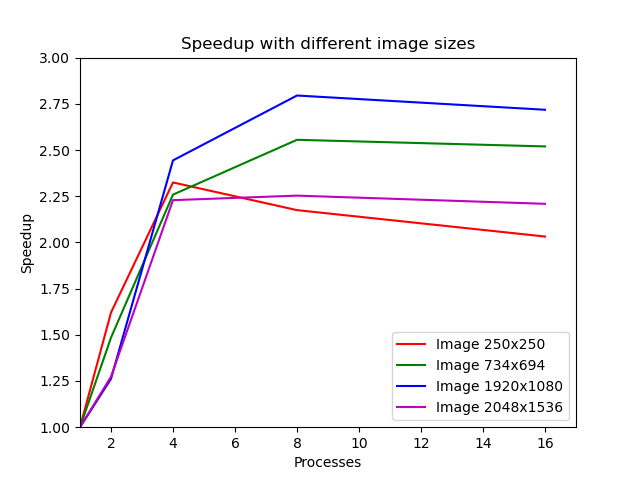
\includegraphics[width=\linewidth]{images/speedup_by_img_sizes.png}
	\caption{Speedup of the LBP operator with $P=8$, $R=1$ with different image sizes.}
	\label{fig:speedup_img}
\end{figure}

\begin{table}[H]
	\begin{center}
		\begin{tabular}{|c|c|c|}
			\hline
			Processes & Execution Time (s) & Speedup \\
			\hline
			1 & 5.218 & 1.000 \\
			2 & 3.220 & 1.620 \\
			4 & 2.245 & 2.324 \\
			8 & 2.399 & 2.175 \\
			16 & 2.568 & 2.032 \\
			\hline
		\end{tabular}
	\end{center}
	\caption{Execution Times for the 250x250 image.}
	\label{tab:speedup_k_i_1}
\end{table}

\begin{table}[H]
	\begin{center}
		\begin{tabular}{|c|c|c|}
			\hline
			Processes & Execution Time (s) & Speedup \\
			\hline
			1 & 48.630 & 1.000 \\
			2 & 32.759 & 1.484 \\
			4 & 21.531 & 2.259 \\
			8 & 19.032 & 2.555 \\
			16 & 19.302 & 2.519 \\
			\hline
		\end{tabular}
	\end{center}
	\caption{Execution Times for the 734x694 image.}
	\label{tab:speedup_k_i_2}
\end{table}

\begin{table}[H]
	\begin{center}
		\begin{tabular}{|c|c|c|}
			\hline
			Processes & Execution Time (s) & Speedup \\
			\hline
			1 & 203.600 & 1.000 \\
			2 & 161.339 & 1.262 \\
			4 & 83.312 & 2.444 \\
			8 & 72.849 & 2.795 \\
			16 & 74.913 & 2.718 \\
			\hline
		\end{tabular}
	\end{center}
	\caption{Execution Times for the 1920x1080 image.}
	\label{tab:speedup_i_3}
\end{table}

\begin{table}[H]
	\begin{center}
		\begin{tabular}{|c|c|c|}
			\hline
			Processes & Execution Time (s) & Speedup \\
			\hline
			1 & 272.129 & 1.000 \\
			2 & 213.772 & 1.273 \\
			4 & 122.107 & 2.229 \\
			8 & 120.782 & 2.253 \\
			16 & 123.202 & 2.209 \\
			\hline
		\end{tabular}
	\end{center}
	\caption{Execution Times for the 2048x1536 image.}
	\label{tab:speedup_i_4}
\end{table}

TODO
%In Figure \ref{fig:speedup_img} we have the speedup trends for different input images. As before, the values increase up to 4 processes and decrease afterwards.
%
%Bigger images tend to have less speedup overall, but still around 2 for more than 4 processes, making the parallel algorithm still more convenient than the sequential one.

\end{document}
